% Titre de la partie
\section{\sndpti}

%%%%%%%%%%%%%%%%%%%%%%%%%%%%%%%%%%%%%%%%%%%%%%%%
% Première diapo
%%%%%%%%%%%%%%%%%%%%%%%%%%%%%%%%%%%%%%%%%%%%%%%%
\begin{frame}
\frametitle{\sndpti}
\framesubtitle{Méthode SPH}

\centering {\huge \sndpti}

\end{frame}


%%%%%%%%%%%%%%%%%%%%%%%%%%%%%%%%%%%%%%%%%%%%%%%%
% Deuxième diapo
%%%%%%%%%%%%%%%%%%%%%%%%%%%%%%%%%%%%%%%%%%%%%%%%
\begin{frame}
\frametitle{\sndpti}
\framesubtitle{Méthode SPH}

\centering
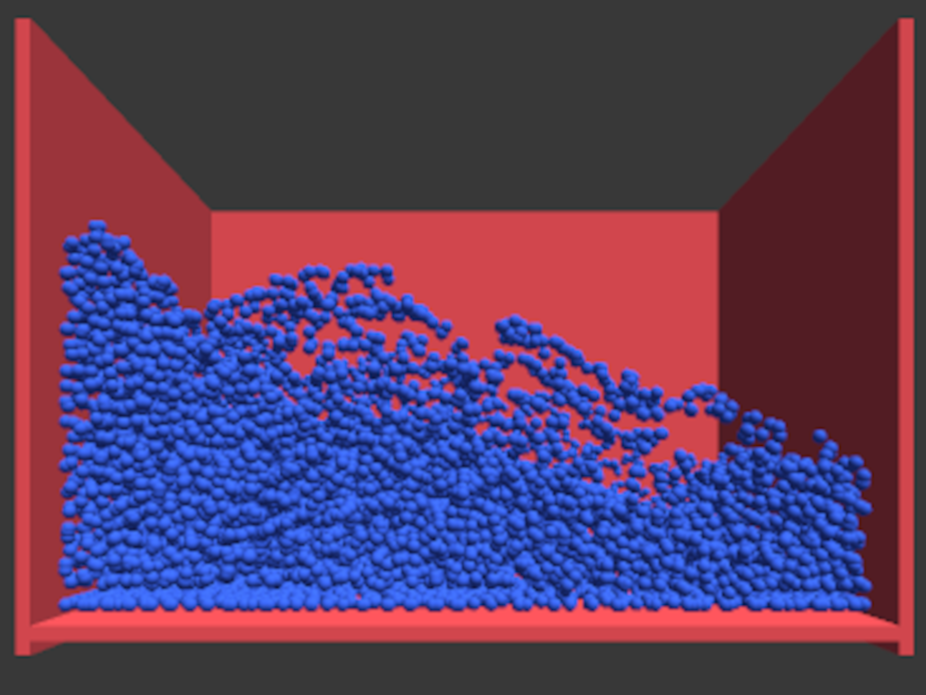
\includegraphics[width=.7\linewidth]{figures/sph_illustration.png}

\end{frame}

%%%%%%%%%%%%%%%%%%%%%%%%%%%%%%%%%%%%%%%%%%%%%%%%
% Troisième diapo
%%%%%%%%%%%%%%%%%%%%%%%%%%%%%%%%%%%%%%%%%%%%%%%%
\begin{frame}
\frametitle{\sndpti}
\framesubtitle{Avantages de cette technique}

\begin{itemize}
    \item Respect de l'équation de conservation de la masse
    \item le terme d'advection est nul 
\end{itemize}
$$(\vec{v}\cdot \vec{\text{grad}}) (\vec{v}) = 0$$

\end{frame}

%%%%%%%%%%%%%%%%%%%%%%%%%%%%%%%%%%%%%%%%%%%%%%%%
% Quatrième diapo
%%%%%%%%%%%%%%%%%%%%%%%%%%%%%%%%%%%%%%%%%%%%%%%%
\begin{frame}
    \frametitle{\sndpti}
    \framesubtitle{Les équations que nous font résoudre cette méthode}
    
    On doit donc juste résoudre:
    $$
    \rho \frac{\partial \vec{v}}{\partial t}= \rho \vec{g} - \vec{grad} P + \eta \Delta \vec{v} + \vec{F}
    $$
    
\end{frame}


%%%%%%%%%%%%%%%%%%%%%%%%%%%%%%%%%%%%%%%%%%%%%%%%
% Cinquieme diapo
%%%%%%%%%%%%%%%%%%%%%%%%%%%%%%%%%%%%%%%%%%%%%%%%
\begin{frame}
    \frametitle{\sndpti}
    \framesubtitle{Obtiention des approximations: prérequis - pseudo-fonction de Dirac}

    \begin{tcolorbox}
        La pseudo-fonction de Dirac:
        \begin{align*}
            \delta(x) =
           \begin{cases}
             + \infty & \text{si } x=0 \\
             0 & \text{sinon}
            \end{cases} \\
            \int_{-\infty}^{+\infty} \delta(x)dx = 1
           \end{align*}
    \end{tcolorbox}

    
\end{frame}


%%%%%%%%%%%%%%%%%%%%%%%%%%%%%%%%%%%%%%%%%%%%%%%%
% Sixième diapo
%%%%%%%%%%%%%%%%%%%%%%%%%%%%%%%%%%%%%%%%%%%%%%%%
\begin{frame}
    \frametitle{\sndpti}
    \framesubtitle{Obtiention des approximations: prérequis - l'identité du Dirac}

    \begin{tcolorbox}
        L'identité du Dirac:

        $\forall g$ continue et intégrable
        \begin{align*}
            \int_\mathbb{R} g(x)\delta(x-t)dx = g(t)
           \end{align*}
    \end{tcolorbox}

\end{frame}

%%%%%%%%%%%%%%%%%%%%%%%%%%%%%%%%%%%%%%%%%%%%%%%%
% Septieme diapo
%%%%%%%%%%%%%%%%%%%%%%%%%%%%%%%%%%%%%%%%%%%%%%%%
\begin{frame}
    \frametitle{\sndpti}
    \framesubtitle{Obtiention des approximations: prérequis - estimation par noyau}
    \onslide*<1>{
        \noindent
        \begin{minipage}[t]{0.4\textwidth}
            Estimation par noyau:
            $$\hat{f}_h(x) = \frac{1}{nh} \sum_{i=1}^n K(\frac{x - x_i}{h})$$
    
            \begin{itemize}
                \item $h$: paramètre de lissage
                \item $K$: fonction noyau de lissage
                \item $n$: nombre de points
               \end{itemize}
        \end{minipage}%
        \begin{minipage}[t]{0.6\textwidth}
            \adjustimage{width=1.0\textwidth,valign=t,margin=2ex 0ex 0ex 0ex}{figures/kernel_smoother_graph.png}
        \end{minipage}
    }

    \onslide*<2>{ \centering 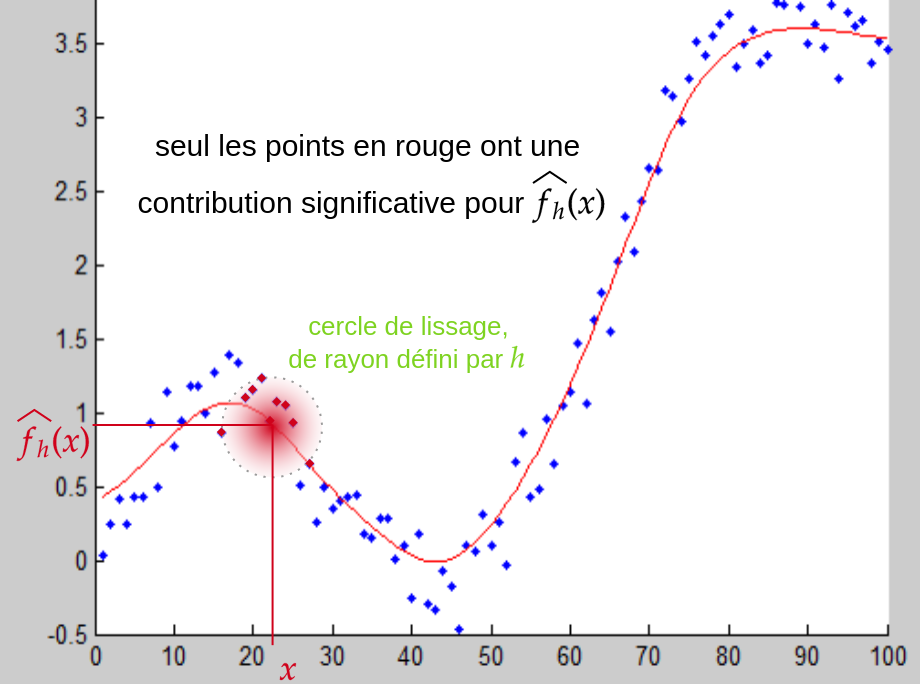
\includegraphics[width=0.8\linewidth]{figures/kernel_smoother_graph.png}}

    \onslide*<3> {
        On pose $\mathbf{q = r/h}$. La fonction $K$ doit répondre à certains critères:
        \begin{align*}
        & \cdot K \text{ positive, définie et décroissante} \\
        & \cdot \lim_{h \to 0}K(r,h) = \delta(r) \\
        & \cdot \sigma \int_{\mathbb{R}^3} f(q)dV = 1
        \end{align*}
    }

\end{frame}

%%%%%%%%%%%%%%%%%%%%%%%%%%%%%%%%%%%%%%%%%%%%%%%%
% Huitieme diapo
%%%%%%%%%%%%%%%%%%%%%%%%%%%%%%%%%%%%%%%%%%%%%%%%
\begin{frame}
    \frametitle{\sndpti}
    \framesubtitle{Expressions dont on doit faire l'approximation}

    \begin{itemize}
        \item<1-> Approximation d'un champs scalaire \\
        \onslide*<2>{
            En posant:
            \begin{align*}
                A(M) = \int_{\mathbb{R}^3} A(M')\delta(\lVert M' - M\rVert)d^3M' \\
                <A>(M) = \int_{\mathbb{R}^3} A(M')K(\lVert M' - M\rVert, h)d^3M'
            \end{align*}
            }
        \onslide*<3>{On se rend compte que:
        \begin{align*}
            A(M) = <A>(M) + O(h^2)
        \end{align*}
        }
        \onslide*<4->{
            \begin{align*}
                A(M) \approx \sum_i \frac{m_i}{\rho_i}A(M_i)K(r_i, h)
            \end{align*}
        }


        \item<5-> Approximation d'un gradient
        \begin{align*}
            \vec{\text{grad}}(A)(M) \approx \sum_i \frac{m_i}{\rho_i}A(M_i) \vec{\text{grad}}(K(r_i, h))
        \end{align*}

        
        \item<6-> Approximation d'un laplacien scalaire
        \begin{align*}
            \Delta A (M) \approx \sum_i \frac{m_i}{\rho_i}A(M_i) \Delta K(r_i, h))
        \end{align*}
    \end{itemize}

\end{frame}

%%%%%%%%%%%%%%%%%%%%%%%%%%%%%%%%%%%%%%%%%%%%%%%%
% Neuvieme diapo
%%%%%%%%%%%%%%%%%%%%%%%%%%%%%%%%%%%%%%%%%%%%%%%%
\begin{frame}
    \frametitle{\sndpti}
    \framesubtitle{Expression discrètes des forces}

    \begin{enumerate}
        \item Densité: $$\rho(M,t) =\sum_i m_i K(r_i, h)$$
        \item Poids: $$\vec{P}(M,t) = \rho(M,t)\vec{g}$$
        \item Pression: $$\vec{F_p}(M,t) = -\sum_i \frac{m_i}{\rho(M_i,t)} p(M_i,t) \vec{\text{grad}}(K(r_i, h))$$
        \item Viscositée: $$\vec{F_{v}}(M,t) = \eta \sum_{j=1}^3 \sum_i m_i \frac{v_i}{\rho(M_i,t)} \Delta K(r_i, h)\vec{u_j}$$
    \end{enumerate}

\end{frame}
